\chapter{Julia}
\label{ch:Julia}
Julia is a new programming language that was created by Jeff Bezanson, Alan Edelman, Stefan Karpinski and Viral B. Shah at Massachusetts Institute of Technology (MIT) \citep{juliaLab}. The language was created in 2009, but was first released publicly in 2012. In 2012 \cite{juliaBlogRelease2012} said in a blog post:
\blockquote{We want a language that’s open source, with a liberal license. We want the speed of C with the dynamism of Ruby. We want a language that’s homoiconic, with true macros like Lisp, but with obvious, familiar mathematical notation like Matlab. We want something as usable for general programming as Python, as easy for statistics as R, as natural for string processing as Perl, as powerful for linear algebra as Matlab, as good at gluing programs together as the shell. Something that is dirt simple to learn, yet keeps the most serious hackers happy. We want it interactive and we want it compiled. (Did we mention it should be as fast as C?)}

\section{Characteristics of Programming languages}
To understand why the creators of Julia wanted to build this new programming language, we need to have a closer look at what type of programming languages are out there already, and what separates them. All programming languages that are used in numerical applications are written in a high level language. This is a language that is easily readable for a human. The code that is written is called source code. This source code needs to be translated for the machine to understand it. The translated code is called machine code. How this translation happens is a big part of what gives the different languages different capabilities. I will not go very deep into the subject, as it is too comprehensive for this thesis, but try to scratch the surface such that the different capabilities of the different languages becomes clear.

\subsection{Type Checking}
Firstly, before the translation happens, the program needs to be type checked. This consist of verifying that the variables are not set to unsupported types. For example, a simple array consisting of integers cannot suddenly at a point in the program hold a string in one of its elements. There are two ways of type checking, the first is called static and the second is called dynamic. In a static language each variable needs to have a defined type beforehand and they are checked before the program is executed. We say that type checking happens before run-time. In addition a variable that is declared as one type cannot change type in its scope. The scope of a variable can quickly be explained as the part of the program where the variable is functioning. In dynamic languages the types of the variables do not need to be known before run-time. Type correctness is checked at run-time, or in other words, continuously as the code is executed. A variable can also change type in its scope. Static languages are faster in the execution since it does not need to check for types as it is already done. You will, however, have to wait for the type checking to finish before the program can be executed. Dynamic languages are slower but the continuous type checking enables language designs that optimizes the coding process such that you can implement your program with less code. The first and most obvious difference from static languages is that you do not have to define what types each variable is. The type checking will find this out on its own at run-time. In addition it opens up for a feature called metaprogramming. Metaprogramming is programs that can take in other code as input and modify it such that implementing your code can be done more efficiently and faster. More specifically how this can be used will be discussed closer in \autoref{sec:Metaprogramming}.

\subsection{Compiled and Interpreted Languages}
The next translation difference between the languages is whether it is compiled or interpreted. A compiled language translates the source code to machine code before run-time while an interpreted language translates the code at run-time. To visualize how run-time compilation works, you can say that for each line of code it is first translated and then executed. Compiled languages are faster in the execution than an interpreted language. The reason for this is that when it translates all the code beforehand it can optimize the code that will be executed. You will, however, have to wait for the compiler to finish translating before the program can be executed. Hence, using an interpreted language can be faster when developing programs, as you do not have to recompile your entire program every time you have made a small change. There is also a third way to translate source code into machine code, called just-in-time compilation (JIT compilation). JIT compiled languages is a combination of compiled and interpreted languages. It compiles blocks of the source code such that it can do optimizations like compiled code, but at the same time it does not need to compile the whole source code before it executes the program. In this way it behaves like an interpreted language, but with the speed advantages of compiled languages. In most cases however, it will be slower than regular compiled languages. Disadvantages for JIT compiled languages is extra memory usage and that writing a JIT compiler is more difficult than other compilers. The latter does not affect the end user of the language.

\subsection{Languages for Numerical applications}
\label{sec:numericalLang}
For numerical applications we can separate the most commonly used languages into two groups. The first group is static and compiled languages like C and C++. These are languages that execute very fast but the time it takes to make the programs are longer. The second group are dynamic and interpreted languages like the well known MATLAB and Python (in 2015 MATLAB introduced a new execution engine that uses JIT compilation \emph{\citep{MatlabJIT}}. However, MATLAB is still a dynamic language that function like a fully interpreted language). These languages are easier to use if you want to create numerical simulations, but they execute slower than C and C++. Julia is a dynamic, but (JIT)compiled language. As the creators said in the blog post from 2012: Julia is supposed to have \enquote{(...) familiar mathematical notation like Matlab}, be \enquote{(...) as  powerful  for  linear  algebra  as Matlab} and at the same time be as fast as C. Summed up their goal has been to make a language that is as easy to use as an interpreted and dynamic language, but with the speed of a compiled and static language. Based on this description, Julia seems to be the perfect language for numerical simulations.

\subsection{Source Code Example}
So far in this chapter, I have discussed what separates the languages concerning type checking and how the source code is translated to machine code. These differences will in return affect the syntax of the languages and how we can write the source code. Below I have an example illustrating different implementations of an example in Julia, MATLAB and C++. The example consist of writing a program that creates two random vectors of length $n$, element-wise multiply them together and print the resulting vector in a readable way. This example is first implemented in Julia, where the random vector is created using \texttt{rand(n)}, the element-wise multiplication is performed with the \texttt{.*} operator and the result is printed with the \texttt{println(...)} function:
\lstinputlisting{code/dot_product.jl}
Very similar to the Julia implementation we have the same program in MATLAB:
\lstinputlisting{code/dot_product.m}
The implementations only have a couple of small syntax differences, and they both implement the example efficiently with few lines. C++ on the other side is not created specifically for mathematical programming and without importing any external libraries (except from \texttt{iostream}, which is needed to print the result), the implementation of the example becomes much more comprehensive:
\lstinputlisting{code/dot_product.cpp}
The first obvious difference is that C++ is not a scripting language like MATLAB and Julia. This means that code we want to execute, needs to be inside a function. This could contribute making the implementation of new code more tedious in C++, than in MATLAB and Julia. From the declaration of the variables, it is clear that C++ is a static language, where each variable needs to have a predefined type. Lastly there are no built in functions to create a random vector, element-wise multiply vectors nor printing vectors. These operations needs to be implemented and shows how C++ is a lower-level language than MATLAB and Julia.

You could argue that this comparison is unfair for C++, as you would either import libraries that have functions to create random vectors, do element-wise multiplication and print vectors, or you would overload operators to do this. By either using such libraries or implemented operators, we would be able to implement the example more compact like in Julia and MATLAB. However, the implementations above are not built in, and they need to be implemented. This can either be done by importing an external library that has implemented this already or by overloading the operators yourself. Hence, the example illustrates some of the differences between two languages that are created with mathematical programming in mind and a language that is not.

\section{History of Julia}
The process of creating a new programming language is long. In 2009 the creators began the project of creating Julia and in the blog post \emph{\citep{juliaBlogRelease2012}} from 2012 they said \enquote{It's not complete, but it's time for a 1.0 release — the language we’ve created is called Julia}. In a new blog post from August 8. 2018 \emph{\citep{juliaBlogReleaseV1.0}}, where they released the actual version 1.0 they admitted that they had jumped the gun a little with the mentioning of v1.0 in 2012, as it took more than six years before it actually happened. But after almost ten years of development v1.0 of the Julia language was released. The major consequence of a 1.0 release is that from this version and on, they guarantee backward compatibility. When they did not guarantee backward compatibility, code that worked on version, 0.1, 0.2, etc., would not necessarily run on newer versions of Julia. But from v1.0, all code that run on this version, will also run on future releases. This was a huge milestone for the Julia language. 

A consequence of the non backward compatibility is that when you search the internet for help in Julia, currently less than one year after the v1.0 release, you could end up finding solutions to your problem that no longer works. Hence, as of now you need to be careful and check the date of the answers, and keep in mind, if it is from before v1.0, it might no longer work. This can at some times be frustrating, especially when you try to learn the language. However, now that there is backward compatibility for future releases, as time goes by, this problem will disappear as pre-v1.0 answers will eventually drown by post v1.0 answers.

Since Julia is an open source and free program to use, one of its strengths is that developers can contribute by creating useful programs that they share with all the other users. One example of this is the Integrated Development Environment (IDE), \cite{JunoIDE}. Juno is a program to help writing Julia code easier and is created by mainly two developers, Sebastian Pfitzner and Mike J. Innes. Juno gives the coder an environment where it is easy to run your Julia code, you get auto completion when writing your code, it has built in plotting panes to visualize results, and much more. The program is open source and free to use, and if you look at \cite{JunoGithub}, there are many other contributors to the IDE other than Pfitzner and Innes. These are developers that have either found an error in the existing code or made a feature they wanted for the IDE. This shows the strength of the code being open source -- the community can contribute to the code database. This will help finishing improvements and error corrections to the code database quicker. This is why v1.0 of Julia was such a milestone, because as soon as Julia has guaranteed backward compatibility, there is a lot easier for developers to justify spending time to develop programs for Julia. This is because the developers now know that the work they put in writing Julia code, will not be in vain, as the code will work on all future releases of Julia. 

\section{Metaprogramming in Julia}
\label{sec:Metaprogramming}
In the last year there have been published numerous projects that makes coding in Julia easier. A lot of these projects exploit that Julia is a dynamic language and that it has metaprogramming. In the blog post from \cite{juliaBlogRelease2012} the creators says that Julia shall contain true macros like the programming language Lisp \emph{\citep{Lisp}}. Macros are functions that are using metaprogramming to modify your existing code to give extra functionality. The macro functions in Julia are easily recognized by an "@" in front of the function name. To use a macro function on any function, you simply call the macro function before the original function call. I will now show four examples of macro functions in Julia that are very useful when creating numerical simulations.
\subsection{Profiling}
\label{sec:profiling}
Profiling is an effective method to obtain overview of where bottlenecks lie in a code when trying to optimize its performance. The method consists of taking snapshots of the code with small time intervals and for each snapshot we register what function we are at and all the functions that have been called to get to this function. The latter is called the stack trace. By counting how many times a function is in the stack trace, we get an overview of how much time we spend in each function and where they are called from. Since we only register the number of times we have observed that we are in each function, this will not give a perfect picture on how much time we spend on all function. We even risk not registering all functions we use, but since the time interval between the snapshots are small (e.g. every tenth microsecond), a function that is not registered will not be interesting to optimize as it is already very fast. 
\begin{figure}[htb]
    \centering
    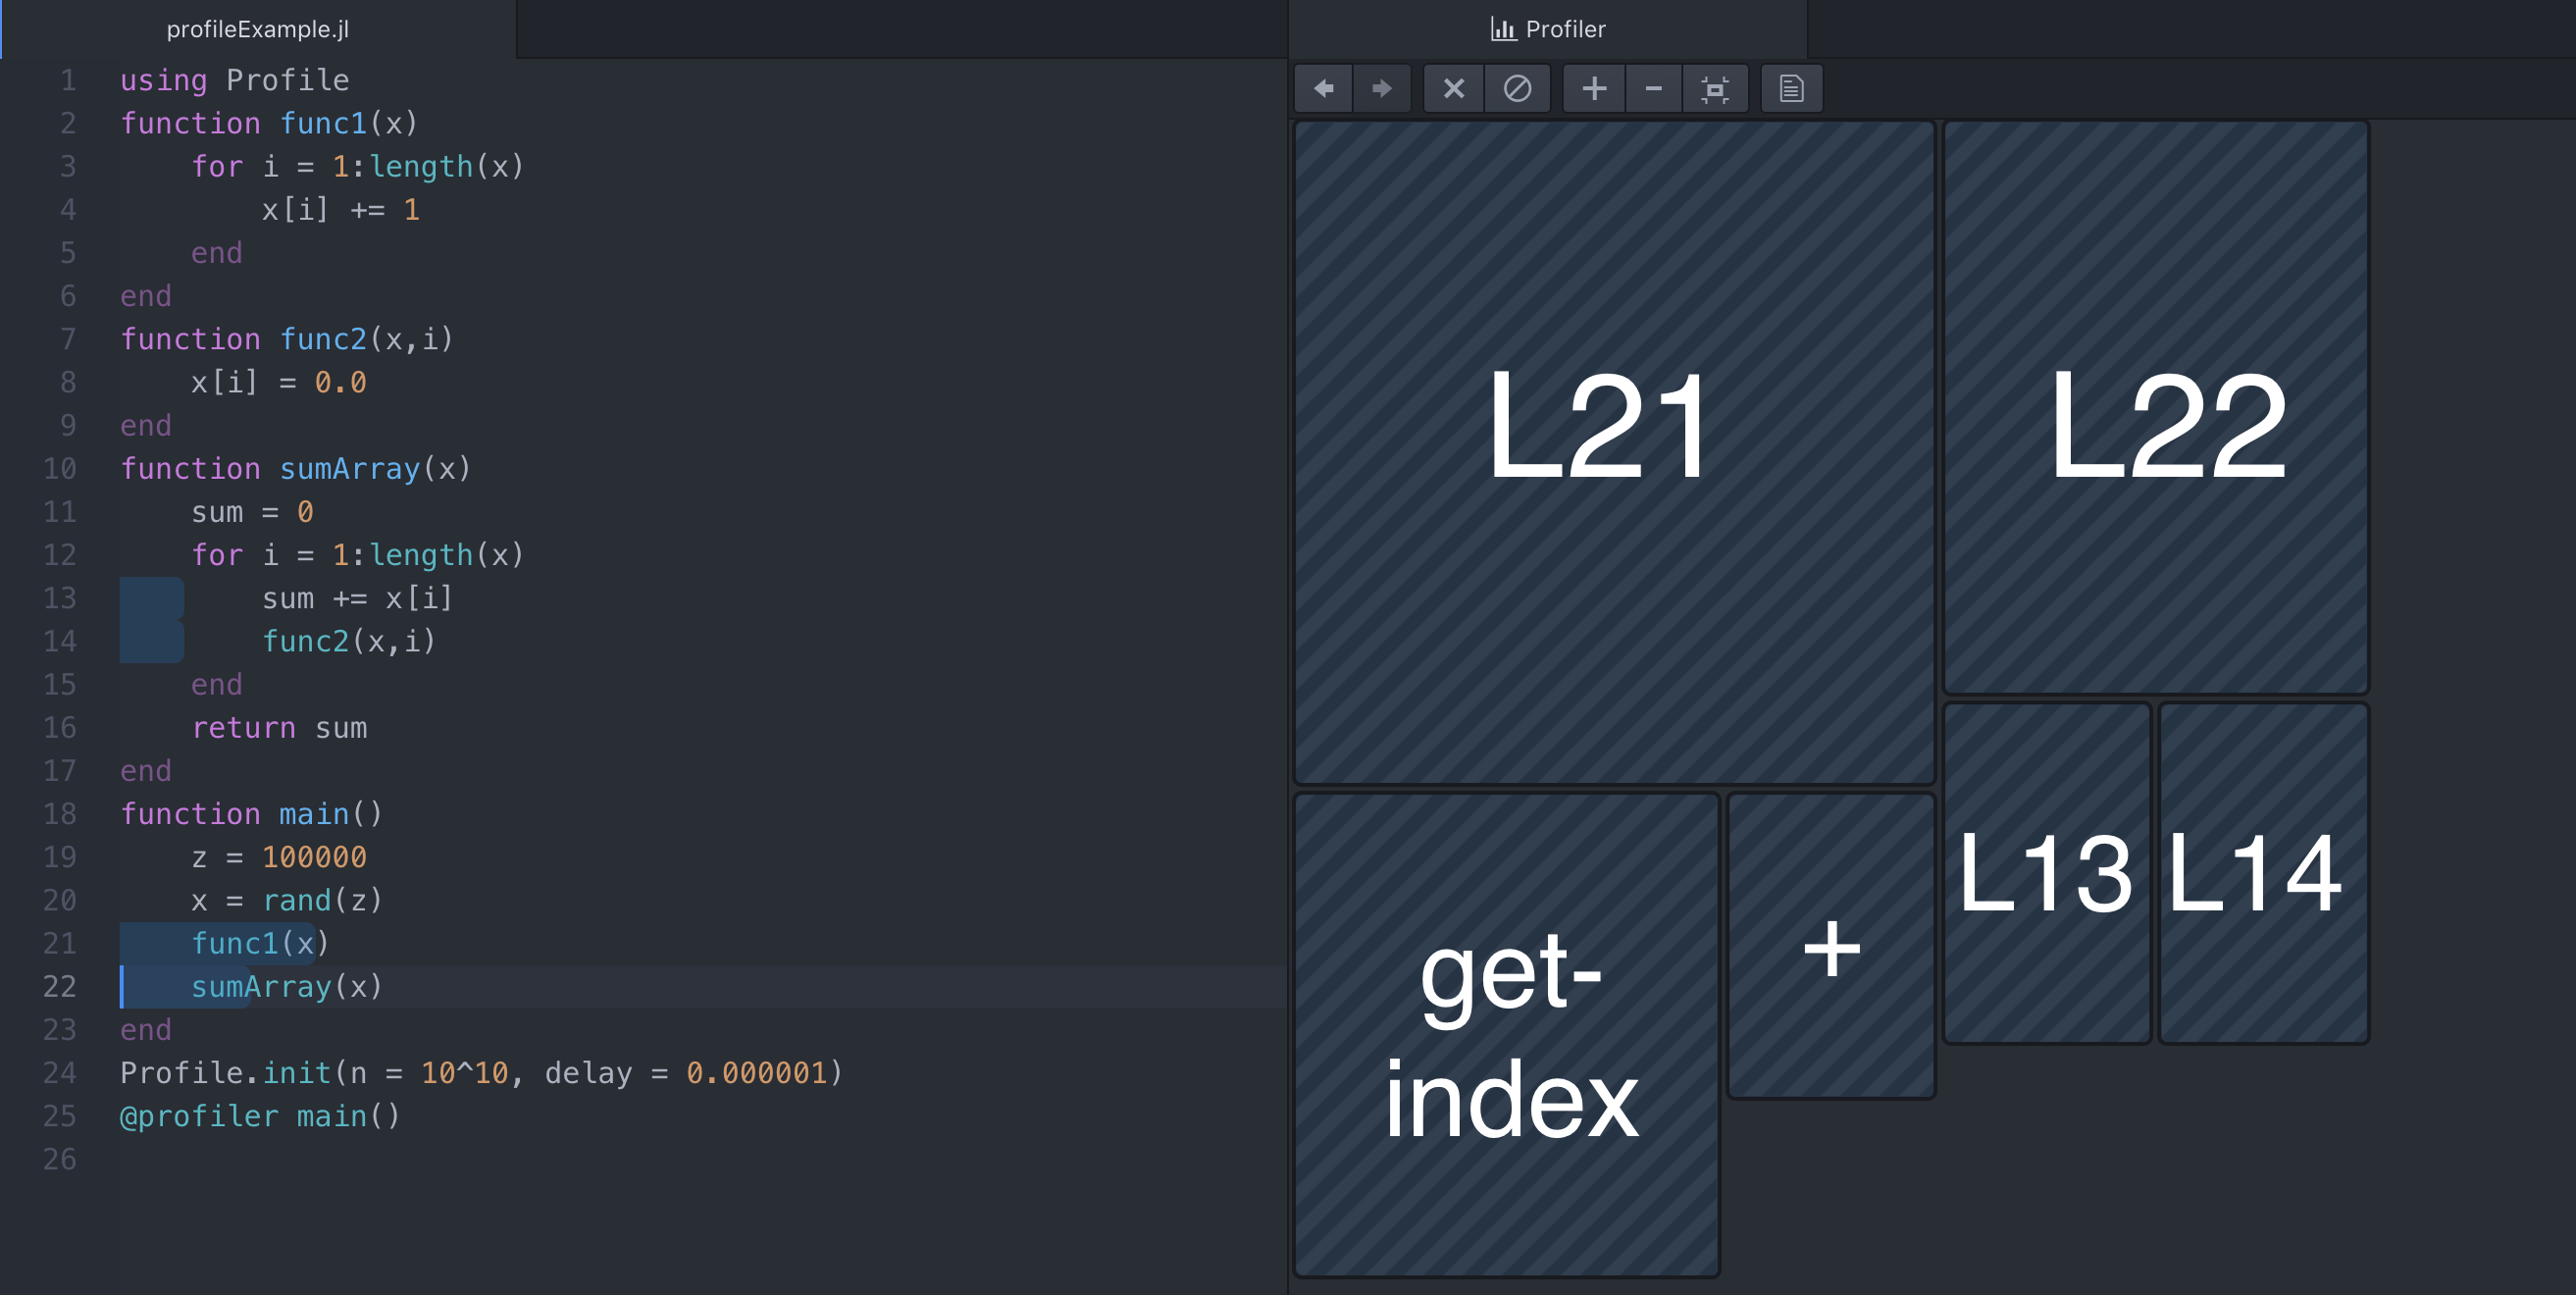
\includegraphics[width = \textwidth]{figures/profiling_screenshot.png}
    \caption{Interface in Juno of the \texttt{@profiler} macro tool for a simple test case. The left hand side shows the code profiled and the right hand side shows the result visualized. Since the visualization is interactive I have added extra text to show which block represents which line in the code.}
    \label{fig:profilingExample}
\end{figure}

\autoref{fig:profilingExample} shows the interface from the Juno IDE using the \texttt{@profiler} macro function \emph{\citep{JunoProfilerMacro}} for a simple test case. The left hand side of \autoref{fig:profilingExample} shows a test case with a \texttt{main()} function that creates a random variable \texttt{x} of length \texttt{z}. It then  calls the \texttt{func1(x)} function that adds 1.0 to each element of \texttt{x}. Lastly it calls \texttt{sumArray(x)} that sums up all the values of \texttt{x} and uses \texttt{func2(x,i)} to set all values of x to zero. \texttt{@profiler} is a specific Juno macro that uses the built in \texttt{@profile} in Julia \emph{\citep{Profile.jl}} to profile the \texttt{main()} function, but in addition it creates the right hand side of \autoref{fig:profilingExample} which shows the profiling result. Since the Profiler pane is interactive, I have added extra white text for visualization. Each block represents one specific operation inside the code and the wider the block is, the more time is spent in that operation. The vertical axis represents how deep into the stack trace the operation is. For \autoref{fig:profilingExample} line 21(L21) and 22 (L22) are at top of the stack trace. We can also see that we spend more time in \texttt{func1(x)} than \texttt{sumArray(x)}. The time spent on each line can also be seen by the blue bars on each line. If we say  L21 and L22 is at depth 1, then line 13 and 14 is at depth 2. The \texttt{getindex} and \texttt{+} blocks are built in functions in Julia that are called from line 4 in \texttt{func1(x)}. These functions are deeper than line 13 and 14 at depth 3. Technically it should have been an extra block underneath line 21 that represents line 4 to get the full stack trace. The only reason I have found why this is not part of the visualization is that the \texttt{@profiler} tool is still a work in progress, and that it does not work perfectly just yet. However, this tool is super efficient to find bottlenecks in your code, especially when you have a larger program than the simple example in \autoref{fig:profilingExample}. 
\subsection{Debugger}
\label{sec:debugger}
Many IDEs for different languages have the ability to debug code. This is a tool to step into your functions and execute them step by step to reveal error and bugs in your code. Recently, on March 19th, \citet{Debugger} published a debugger for Julia. This can be used directly in the terminal using the \texttt{@enter} macro function or as a built-in debugger in Juno with \texttt{Juno.@enter}. \autoref{fig:debuggerExample} shows the interface of Juno's debugger for a simple test function.
\begin{figure}[htb]
    \centering
    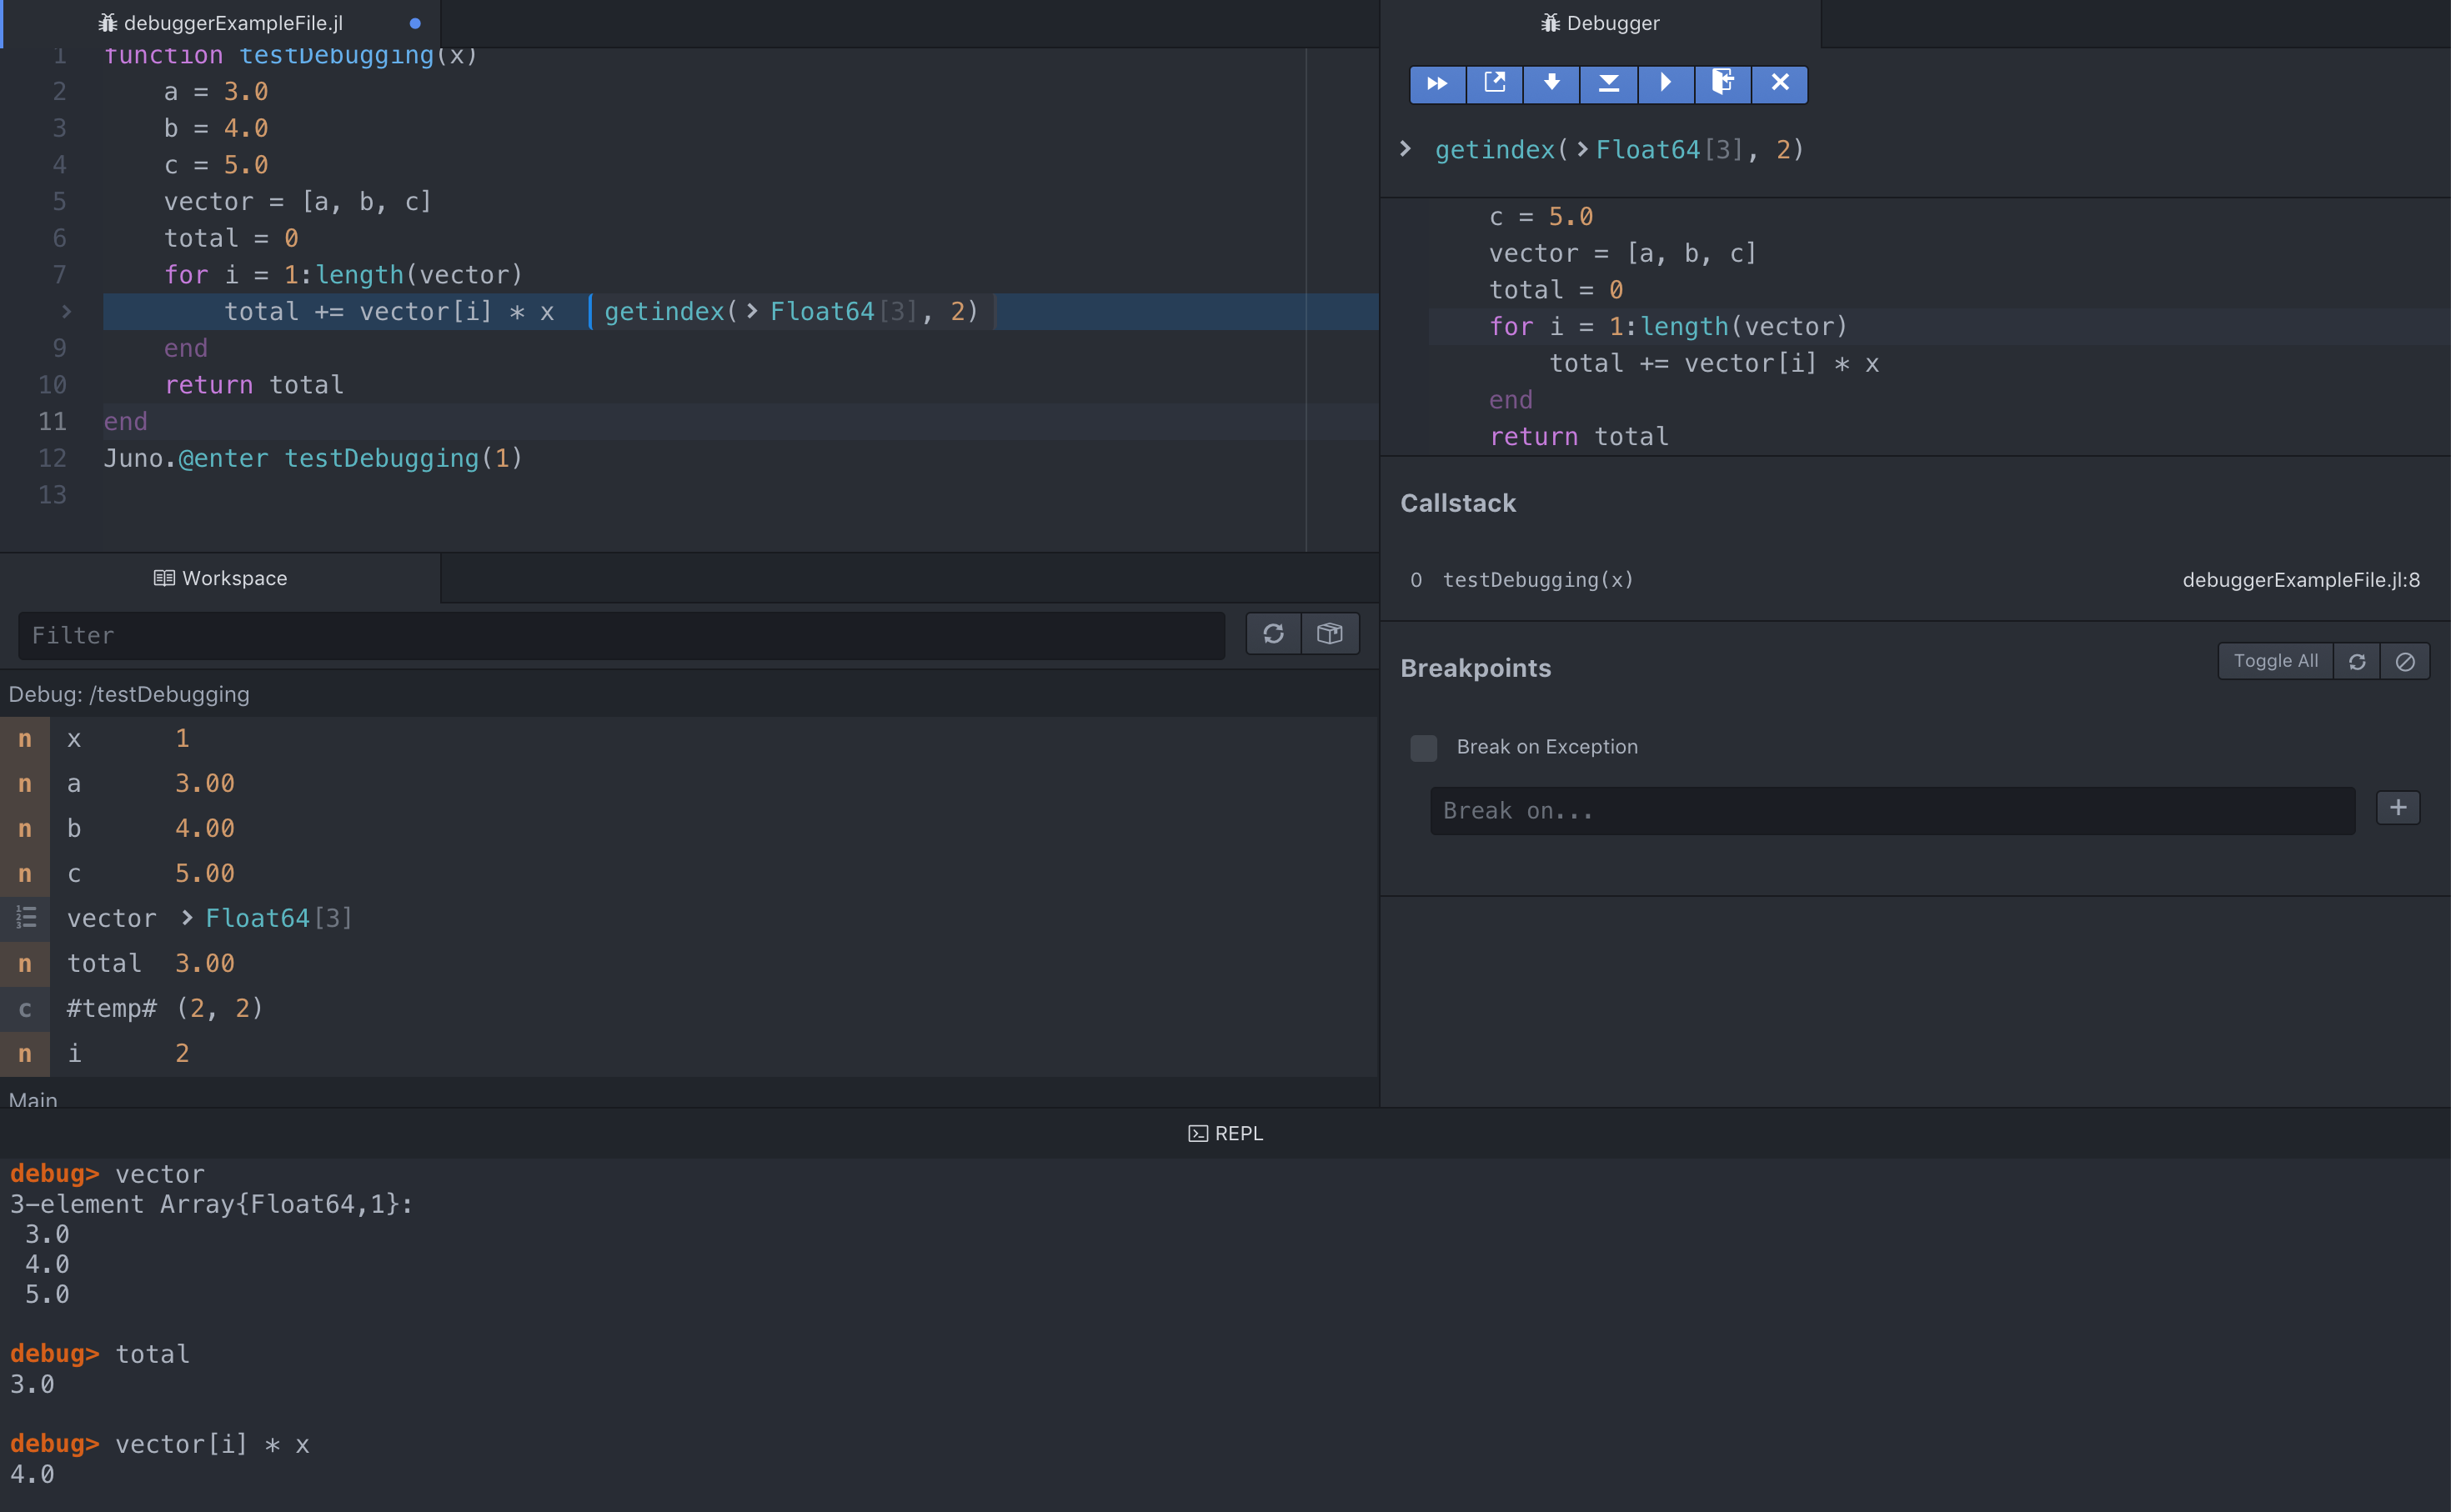
\includegraphics[width = \textwidth]{figures/debugger_screenshot.png}
    \caption{Juno's interface in debugging mode.}
    \label{fig:debuggerExample}
\end{figure}
With this you have the opportunity to:
\begin{itemize}
    \item Execute the code, step by step.
    \item See the next function or operation that will be executed.
    \item See the values of the variables in the workspace.
    \item Work with the variables from the workspace at their current state.
    \item See the current call stack (or the stack trace) which shows how you got to this part of the code.
    \item Set breakpoints such that you can execute your code until the breakpoint.
    \item Make corrections to the code that will impact the execution of the code immediately.
\end{itemize}
The opportunity to use a debugger to find bugs and correct your code can be very valuable and in some scenarios save the programmer a lot of time. 

\subsection{Benchmarking}
\label{sec:benchmarking}
When writing code for numerical simulations, or any other code for that matter, it is interesting to benchmark the simulation. Benchmark will in this thesis refer to testing the time spent to execute the function and the memory usage and compare it to other alternative implementations. Julia has a built in \texttt{@time} macro function \emph{\citep{@time}} that returns the time spent to execute the function together with the number of memory allocations and total memory used. This is a great tool, but especially time can be difficult to measure accurately. This is because there are numerous of other processes happening on your computer that there is impossible to control. Examples of this can be that you might get an email while you execute your code or the computer decides to take backup of some of your files. All these uncontrollable factors can affect the time spent to execute a simulation. 

An option to reduce possible sources of errors is to run the benchmark multiple times and use the average time spent. However, then you have to write this extra code every time you want to benchmark a function. \emph{\cite{BenchmarkTools}} is a library that gives you a macro function called \texttt{@btime} that does exactly this so that you do not have to write repetitive code. It uses \texttt{@time} multiple times to get a result that is less prone to sources of errors. The primary macro function from \textit{BenchmarkTools} is however \texttt{@benchmark} which returns minimum, maximum, mean and average time, together with memory allocation and usage, and information on how many samples it has taken. All this is easy to use because of Julia's metaprogramming. It makes it quick and safe to benchmark all types of simulations and codes, without repeating your source code.

\subsection{Parallel Computing}
\label{sec:parallelComputing}
Parallel computing is wide topic that can be performed at many levels. However, the main idea is to split a task into smaller problems and execute them simultaneously. New computers are delivered with multi-core processors, giving them the ability to perform multiple tasks simultaneously. The speedup for programs using parallel computing compared to regular linear computing can be up to the number of cores, and in best case scenarios, the speedup can actually be even more than the number of cores. In these cases the extra speedup is an effect caused by the memory allocation becoming easier when the task executed is split up into smaller problems. However, for the computer to be able to perform parallel computing, the source code needs to be written such that it supports parallelization. This parallelization of the code is important, because even though the possible computational gain from parallelization can be huge, a bad written parallel code can execute slower than the linear equivalent. 

In Julia, parallel computing is implemented using metaprogramming \emph{\citep{ParallellComputing}}. There are different types of parallel programming that are implemented, but I will focus on what is called multi-threading. Multi-threading means that we have different threads that perform different tasks simultaneously. By using the \texttt{Threads.@thread} macro in front of a for-loop, Julia will automatically split the different iterations between all the available processing cores. The Julia documentation has a good example on how this works. The example consist of initializing a vector, \texttt{a}, containing only zeros and loop through it. The iterations are happening in parallel and each element in \texttt{a} becomes the identification number of the core that performed the iteration. The example code can be seen below:
\lstinputlisting{code/threads.jl}
In the last line, the output of \texttt{println(a)} is commented. We can see that the example has been executed with four available cores, and that each core has performed two iterations. This use of metaprogramming to parallelize code is very elegant and makes parallelization of code very easy. However, as warned in the Julia documentation, the implementation of multi-threading is, at the moment of writing this thesis, experimental. This means that it can work for some examples and for others it will crash and not work. For the simple example displayed above, it will work, but for more extensive examples, the program will crash. The use of multi-threading has been tried applied to the methods described in this thesis, but unfortunately the multi-thread macro functions are too unstable to handle these cases. However, it is an interesting feature to look into when the development has come further and the macro functions are more stable. 

Subsection \ref{sec:profiling}, \ref{sec:debugger}, \ref{sec:benchmarking} and \ref{sec:parallelComputing} are all great examples of how powerful tools, that help developers code, are being created less than a year after v1.0 of Julia was released. This community, together with the ideas of a very fast language, makes Julia a very interesting language to try out and to see what is possible to achieve concerning easiness of code writing and execution performance.